\documentclass[../main.tex]{subfile}
\graphicspath{{\subfix{../images}}}
\begin{document}

深度网络已经被用于物体检测。我们简要回顾一下最近最先进的R-CNN方法[7]。R-CNN首先通过选择性搜索[20]从每个图像中提取大约2000个候选窗口。然后,每个窗口中的图像区域被扭曲成一个固定的大小($227\times 227$)。一个预先训练好的深度网络被用来提取每个窗口的特征。然后在这些特征上训练一个二分类SVM分类器进行检测。R-CNN产生的结果具有令人信服的质量,大大超过了以前的方法。然而,由于R-CNN将深度卷积网络重复应用于每张图像的约2000个窗口,因此很耗时。特征提取是测试中的主要时间瓶颈。

\begin{figure}[htb]
    \centering
    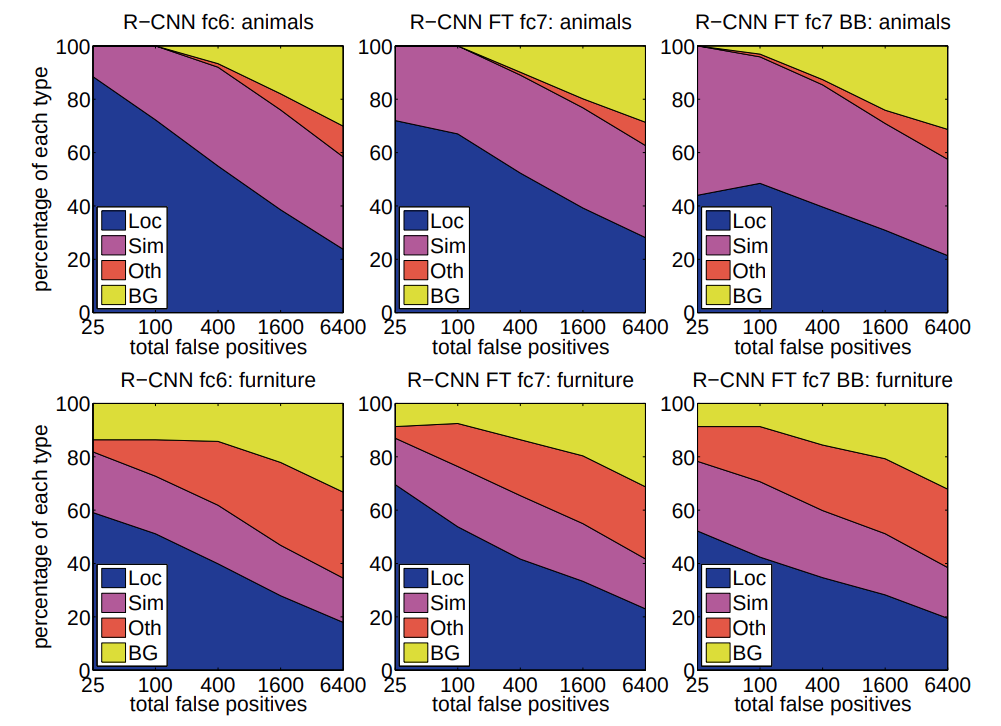
\includegraphics[width=\textwidth]{fig5.png}
    \caption{将特征图上的任意窗口的特征汇集。特征图是由整个图像计算得到的。池化是在候选窗口中进行的。}
    \label{fig:fig5}
\end{figure}

我们的SPP-网络也可用于物体检测。我们只从整个图像中提取一次特征图(可能是多尺度的)。然后,我们在特征图的每个候选窗口上应用空间金字塔池化,以池化这个窗口的固定长度表示(见图\ref{fig:fig5})。因为耗时的卷积只应用一次,所以我们的方法运行速度可以快上几个数量级。

我们的方法是从特征图的区域中提取窗口的特征,而R-CNN则是直接从图像区域中提取。在以前的工作中,可变形部分模型(DPM)[23]从HOG[24]特征图的窗口提取特征,选择性搜索(SS)方法[20]从编码的SIFT特征图的窗口提取。Overfeat检测方法[5]也是从深度卷积特征图的窗口中提取,但需要预先定义窗口大小。相反,我们的方法可以从深度卷积特征图的任意窗口中提取特征。

\subsection{检测算法}

我们使用选择性搜索的 "快速 "模式[20],为每幅图像生成约2,000个候选窗口。然后我们调整图像的大小,使$\min\left(w, h\right) = s$,并从整个图像中提取特征图。我们暂时使用ZF-5的SPP-net模型(单尺寸训练)。在每个候选窗口中,我们使用一个4级空间金字塔($1\times 1$,$2\times 2$,$3\times 3$,$6\times 6$,共50个仓)来汇集特征。这就为每个窗口生成了12,800维($256\times 50$)的表示。这些表征被提供给网络的全连接层。然后我们在这些特征上为每个类别训练一个二元线性SVM分类器。

我们对SVM训练的实现遵循[20],[7]。我们使用ground-truth窗口来生成正样本。负样本是那些与正样本窗口最多重叠30\%的样本(用交集比(IoU)衡量)。任何负面样本如果与另一个负面样本重叠超过70\%,则被删除。我们应用标准的难负例挖掘[23]来训练SVM。这个步骤迭代了一次。为所有20个类别训练SVM需要不到1小时。在测试中,分类器被用来对候选窗口进行评分。然后我们对打分后的窗口使用非最大抑制[23](阈值为30\%)。

我们的方法可以通过多尺度特征提取来改进。我们调整图像大小,使$\min\left(w, h\right) = s\in S = \left\{ 480, 576, 688, 864, 1200 \right\}$,并计算每个尺度的$\text{conv}_5$的特征图。结合这些尺度的特征的一个策略是逐个通道汇集它们。但我们根据经验发现,另一种策略可以提供更好的结果。对于每个候选窗口,我们选择一个单一的尺度$s\in S$,使得该尺度的候选窗口的像素数最接近$224\times 224$。然后我们只使用从这个尺度中提取的特征图来计算这个窗口的特征。如果预设的尺度足够密集,并且窗口近似于正方形,我们的方法大致相当于将窗口的大小调整为$224\times 224$,然后从中提取特征。尽管如此,我们的方法只需要从整个图像中计算一次特征图(在每个尺度上),而不管候选窗口的数量如何。

我们还按照[7]对我们的预训练网络进行了微调。由于我们的特征是由任何大小的窗口的$\text{conv}_5$特征图汇集而成的,为了简单起见,我们只对完全连接的层进行微调。在这种情况下,数据层接受$\text{conv}_5$之后的固定长度的集合特征,然后是fc6,7层和一个新的21路(一个额外的负类别)fc8层。fc8的权重是用$σ=0.01$的高斯分布初始化的。我们将所有的学习率固定为1e-4,然后调整为所有三个层的1e-5。在微调过程中,正样本是那些与真实窗口$\left[ 0.5, 1 \right]$重叠的样本,而负样本是$\left[ 0.1, 0.5 \right]$。在每个迷你批中,25\%的样本是阳性的。我们用1e-4的学习率训练250k个迷你批,然后用1e-5训练50k个迷你批。因为我们只对fc层进行微调,所以训练速度非常快,在GPU上大约需要2个小时(不包括预先缓存特征图,这需要1个小时)。同样按照[7],我们使用边界盒回归来对预测窗口进行后处理。用于回归的特征是来自$\text{conv}_5$的集合特征(与[7]中使用的$\text{pool}_5$特征相对应)。用于回归训练的窗口是那些与ground-truth窗口重叠至少50\%的窗口。

\end{document}